% DUET -- DAC 2027 submission (double-blind, 6 pages + 1 reference page).
% DAC 2027 guidelines (dac.com/2027/program/research-manuscript-submissions): IEEE template, two columns, 9 or 10 pt,
% references on a separate last page only, room left for the author block, no author info in the PDF metadata.
% Build: latexmk -pdf main.tex
\documentclass[conference,9pt]{IEEEtran}
\usepackage{cite}
\usepackage{amsmath,amssymb}
\usepackage{graphicx}
\usepackage{xcolor}
\usepackage{tikz}
% numbered badges of Figure 4: coarse GC (purple) and fine GC (blue)
\definecolor{cgcol}{HTML}{5B3FA0}
\definecolor{fgcol}{HTML}{1F5FA8}
\newcommand{\gcbadge}[2]{\tikz[baseline=(b.base)]\node[circle,fill=#1,text=white,inner sep=0.5pt,minimum size=1.15em,font=\scriptsize\bfseries\sffamily](b){#2};}
\newcommand{\cgc}[1]{\gcbadge{cgcol}{#1}}
\newcommand{\fgc}[1]{\gcbadge{fgcol}{#1}}
\usepackage[hidelinks,pdfauthor={},pdfcreator={},pdfproducer={}]{hyperref}

\begin{document}

\title{DUET: Dual-Granularity Address Translation for High-Capacity SSDs}   % TODO: final title

% double-blind: placeholder that keeps room for the final author block
\author{\IEEEauthorblockN{Anonymous Author(s)}
\IEEEauthorblockA{Affiliation omitted for double-blind review}}

\maketitle
\suppressfloats[t]  % keep Figure 1 out of the left column, so it goes to the top of the right column

\begin{abstract}
% Numbers = geomean throughput over 10 workloads, results/paper_dac/eval_data.csv (final_vbm).
High-capacity QLC SSDs cannot keep a 4\,KB page-level mapping table in
on-device DRAM. Existing FTLs that fit a limited mapping DRAM budget slow reads
with mapping misses, slow writes with block-level merges, or turn every small write into
a read-modify-write (RMW) of a \emph{uniform coarse indirection unit} (uniform coarse IU). We present
DUET, an FTL that keeps the coarse IU and maps writes smaller than a coarse IU as
4\,KB fine pages in a fixed-size DRAM hash table. When the table fills, DUET
spills the fine-map entries of a coarse IU to NAND instead of moving data, and
it merges fine pages one coarse IU at a time. In NVMeVirt with 1/8 of the
page-level mapping DRAM, DUET reaches 93\% of the throughput of a page-level FTL
with unlimited DRAM, whereas on-demand mapping, block-level hybrid mapping, and a
uniform coarse IU reach at most 73\%, 57\%, and 66\%, respectively.
\end{abstract}

% DUET -- Introduction (DAC 2027 draft, 2026-10-20)
% Numbers: results/paper_dac/tables.md (NVMeVirt, 12.5% mapping DRAM, OP 7%). TODO-marked cites need sources.
% Class numbers: best FTL of each class per workload (on-demand = DFTL, LeaFTL; hybrid = FAST, CoMap; coarse IU = IU+RMW).
% Read 2.4x = min(DFTL, LeaFTL) / DUET avg read, max over workloads (YCSB-B). p99 write 4.6x = FAST / DUET on TPC-C. FAST = FAST-B12 (same budget). FAST full (cache_bytes=1e9, results/final_fastfull): 72%, 2.7x.

\section{Introduction}
\label{sec:intro}

The flash translation layer (FTL) is the SSD firmware layer that maps every
logical page to its physical location. Because NAND flash cannot be overwritten
without erasing a whole block, physical pages are programmed sequentially within
a block and every update is written out of place, so the FTL maintains a mapping
table that translates each logical page to its current physical page. Most
commercial SSDs deployed today map at 4\,KB granularity and keep this table in
on-device DRAM.

With QLC NAND, SSDs of 64 and 128\,TB are being released and
developed~\cite{solidigm-122tb,samsung-bm1743}. At 4\,KB granularity, a 64\,TB SSD has
$2^{34}$ logical pages, so each entry needs at least 34 bits and the table takes
68\,GB. A 128\,TB SSD needs 35-bit entries and 140\,GB. Providing this much
on-device DRAM is impractical because of its cost, power, and board
area~\cite{micron-iu}, so large SSDs have to translate addresses with a
mapping DRAM budget that is only a fraction of the full page-level table
(Figure~\ref{fig:intro}a).

\begin{figure}[t]
  \centering
  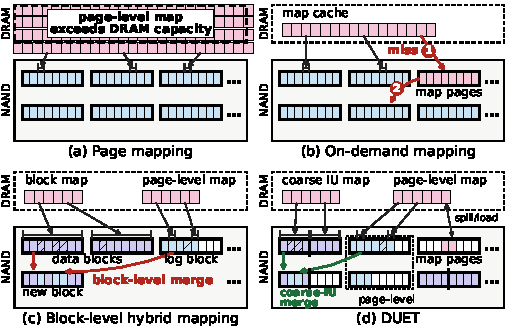
\includegraphics[width=\columnwidth]{figs/fig_intro.pdf}
  \vspace{-6mm}
  \caption{Address translation of four FTLs. In (d), page-level mappings spill to
  map pages instead of being merged when the DRAM table is full, and are loaded back on access.}
  \label{fig:intro}
  \vspace{-2.5mm}
\end{figure}

Techniques that reduce the mapping DRAM fall into two broad classes, and both
pay for it in latency.
\emph{On-demand mapping}~\cite{dftl,leaftl} (Figure~\ref{fig:intro}b) keeps the
page-level table in flash and keeps part of it in an on-device map cache.
A read that misses in the map cache must first read its mapping entry from
NAND before it can read the data. This extra read is synchronous, so read
latency spikes whenever the map cache misses.
\emph{Block-level hybrid mapping}~\cite{bast,fast,janusftl,cftl}
(Figure~\ref{fig:intro}c), on the other hand, maps most data
per NAND block and appends updates to page-mapped log blocks. When free space
runs low, the log blocks are merged back into their data blocks, and a merge
must copy all valid pages of a whole NAND block. Each 3D NAND generation
enlarges the NAND block~\cite{pen}, so a merge copies more pages,
and these copies compete with host writes for NAND bandwidth. In our measurements, the p99 write latency
of FAST~\cite{fast}, a representative block-level hybrid mapping FTL, is 2.8--3.4$\times$ that of a page-level FTL under random I/O.

Many recent commercial high-capacity SSDs instead map all data with a
\emph{uniform coarse indirection unit} (uniform coarse IU) of 16--64\,KB~\cite{micron-iu,solidigm-csal}. The
whole coarse table fits in on-device DRAM, with no mapping misses and no block-level merges.
The cost moves to small writes. When a write is smaller than a coarse IU, the FTL
reads the rest of the unit, merges the new data, and writes the whole unit again
(read-modify-write, RMW). This raises the write amplification (WA) and
lengthens write latency.

We present \textbf{DUET} (\textbf{DU}al-granularity \textbf{E}conomical
\textbf{T}ranslation), an FTL that keeps two mapping granularities, the coarse IU
and the 4\,KB page, under a fixed mapping DRAM budget (Figure~\ref{fig:intro}d). Most data are mapped per coarse IU, and recent writes smaller than a
coarse IU are mapped at 4\,KB granularity. They are written out of place as 4\,KB
pages, and the corresponding pages of the coarse IU become invalid, so the host
write path has no RMW. Most of the page-level mappings stay in on-device
DRAM, and DUET uses NAND only to stage a small part of them so that they fit
the DRAM budget, which is fixed in hardware. DUET thus needs far fewer mapping
reads than on-demand mapping, which reduces its read latency.
When either the page-level or the coarse-IU-level area runs out of
space, its garbage collection (GC) merges the 4\,KB pages of a coarse IU into it and
rewrites the whole coarse IU. A merge rewrites only one coarse IU regardless of the NAND
block size, so DUET never performs the block-level merges of existing hybrid mapping FTLs.

We implement DUET and six other FTLs in NVMeVirt~\cite{nvmevirt}, a kernel-level
NVMe SSD emulator, and evaluate them under a limited mapping-DRAM budget with
microbenchmarks, application workloads, and real-world traces. DUET reaches 93\%
of the throughput of a page-level FTL with unlimited DRAM,
whereas on-demand mapping, block-level hybrid mapping, and a uniform coarse IU reach at most
73\%, 57\%, and 66\%, respectively. Its average read latency is up to
2.4$\times$ lower than that of on-demand mapping, and its p99 write latency is
4.6$\times$ lower than that of block-level hybrid mapping on TPC-C.

This paper makes the following contributions:
\begin{itemize}
  \item An analysis showing that existing FTLs fit a limited mapping DRAM budget only by
  paying in read latency (on-demand mapping), merge cost and tail latency
  (block-level hybrid mapping), or RMW (uniform coarse IU).
  \item The design of DUET, which combines dual-granularity mapping with coarse-IU-level
  merging.
  \item An implementation of DUET and six other FTLs in a common emulator. Under the
  same DRAM budget, DUET achieves the highest average throughput among the
  bounded-DRAM FTLs, within 7\% of a page-level FTL with unlimited DRAM.
\end{itemize}

% DUET -- Background and Motivation (DAC 2027 draft, 2026-10-21)
% Numbers: raw I/O R70, 4K:128K=70:30, 128K-aligned uniform random replay at QD32 (results/final_rp_a128/replay_a128_r70_s70), 1/8 DRAM, OP 7%.
% Figure: results/paper_dac/fig_motiv.pdf (tools/plot_motiv.py).

\section{Background and Motivation}
\label{sec:bg}

\subsection{Address Translation under a DRAM Budget}
NAND flash is read and programmed in pages (4--16\,KiB) but erased only in
much larger blocks, and a page cannot be overwritten before its block is
erased. The SSD controller therefore writes every update out of place and runs
a flash translation layer (FTL) that maps each logical page to its current
physical page. Old copies become invalid, and garbage collection (GC)
reclaims a block by copying its remaining valid pages elsewhere and erasing it.
These copies make the device write more than the host does. The ratio is the
write amplification factor (WAF), and spare over-provisioned (OP) capacity
keeps it bounded.

A page-level FTL keeps one entry per 4\,KiB logical page, so its table is
about 0.1\% of the capacity and grows linearly with it. When the on-device
DRAM can hold only a fraction of this table (1/8 in this paper), the FTL must
either keep part of the mapping in flash or map data in larger units. The
three approaches below take these two routes, and each one moves the cost to a
different part of the I/O path.

\textbf{On-demand mapping.}
DFTL~\cite{dftl} stores the whole page-level table in flash as translation pages
and keeps recently used entries in an on-device \emph{map cache}. A small global
directory locates each translation page. A read that misses in the map cache must first read the
translation page and only then the data page, so two flash reads are
serialized on the read path. Evicting a dirty entry also writes its translation
page back, which adds write amplification. LeaFTL~\cite{leaftl} compresses the
map cache into learned linear segments, so the same DRAM covers more pages.
The segments, however, are built only from runs of sequentially placed pages,
and a mispredicted location costs an extra flash read. For data written randomly
or reordered by garbage collection, both FTLs miss often, and every miss turns
one read into two dependent flash reads. Read latency therefore depends on the
map-cache hit ratio, not on the device.

\textbf{Block-level hybrid mapping.}
Block-level hybrid FTLs such as BAST~\cite{bast}, FAST~\cite{fast}, and
Janus-FTL~\cite{janusftl} map most data per NAND block,
which needs only one entry per block, and absorb updates in a small pool of
page-mapped \emph{log blocks}. When the pool runs out, a log block is reclaimed
by \emph{merging}: for each logical block that has pages in it, the valid pages
from the data block and the log blocks are copied into a fresh block, and the
old blocks are erased. In FAST a log block is fully associative, so one
reclamation can trigger a full merge for every logical block that it touches.
Reads stay cheap, because the block map always fits in DRAM. Merges, however,
run on the write path when no log block is free, so the write that triggers
them waits for several block copies. Each merge copies up to a whole erase
block, and NAND blocks keep growing with every 3D NAND
generation~\cite{TODO-block-size}. The result is long write stalls (write
latency) and many extra copies (write amplification), which together lower
write bandwidth.

\textbf{Coarse-IU mapping.}
High-capacity SSDs in production avoid both problems by using a coarse
\emph{indirection unit} (IU) of 16--64\,KiB~\cite{TODO-iu}. One entry per IU
shrinks the table by the IU size over 4\,KiB, so the whole table fits in DRAM:
every read takes a single flash access, and there are no block merges. The cost
moves to writes smaller than an IU. The FTL must read the rest of the unit,
merge the new data, and program the whole unit again (read-modify-write, RMW).
The extra reads lengthen the write path, and the rewritten pages raise write
amplification by up to the IU size over the write size. In our evaluation the
1/8 budget allows a 32\,KiB IU (4\,B per 32\,KiB), which raises WAF by
2.7--3.3$\times$ over a page-level FTL on YCSB-A and YCSB-B.

\subsection{Motivation}
Figure~\ref{fig:motiv} compares the three approaches with a page-level FTL
that keeps its whole table in DRAM. All FTLs run in NVMeVirt~\cite{nvmevirt}
with the same NAND timing and the same 1/8 mapping-DRAM budget. The workload is
uniform random I/O over the whole device at 70\% reads, and 70\% of the requests are
4\,KiB and the rest 128\,KiB, each aligned to its own size (QD32).

\textbf{On-demand mapping slows reads.}
With mapping misses, DFTL needs 1.37 flash reads per host read and LeaFTL 1.16
(Figure~\ref{fig:motiv}a, where LeaFTL's misprediction reads are not counted, so its
value is a lower bound). Their average read latency is 2.1$\times$ and
1.4$\times$ that of the page-level FTL (Figure~\ref{fig:motiv}b), although the
flash itself is the same.

\textbf{Block-level hybrid mapping and coarse IUs slow writes.}
FAST's block merges raise WAF from 8.6 to 26.5 (Figure~\ref{fig:motiv}c) and
stall writes, so its average write latency is 2.8$\times$ that of the page-level
FTL (Figure~\ref{fig:motiv}d) and it delivers only 37\% of the page-level
throughput. The coarse IU avoids merges, but every 4\,KiB write becomes an RMW of
its 32\,KiB unit: WAF reaches 12.8 (1.5$\times$) and write latency grows by 1.4$\times$.

DUET, shown for reference, uses the same 11.2\,MB as the other bounded FTLs
(1/8 of the page-level table), serves every read here with one flash read, and stays within
1.1$\times$ of the page-level FTL in average read and write latency and WAF.

\textbf{Goal.}
An FTL that fits a limited DRAM budget should therefore (i) minimize mapping
reads, so that a host read costs a single flash read as with a coarse IU,
(ii) eliminate block merges, and (iii) absorb small writes without RMW.
DUET meets all three by keeping the coarse IU and adding a fine-grained level
whose mapping is elastic.

\begin{figure}[t]
  \centering
  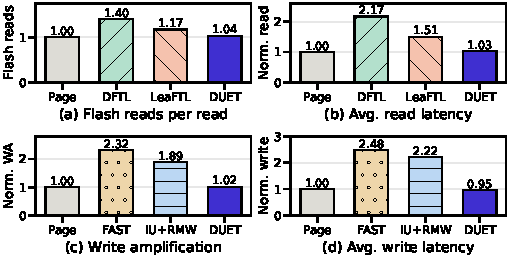
\includegraphics[width=\columnwidth]{figs/fig_motiv.pdf}
  \vspace{-6mm}
  \caption{Cost of existing FTLs under a 1/8 mapping-DRAM budget (uniform random,
  70\% reads, 70\% 4\,KiB / 30\% 128\,KiB size-aligned requests, QD32). (a)--(b)
  On-demand mapping. (c)--(d) Block-level hybrid mapping (FAST) and a 32\,KiB coarse IU with RMW.
  Latencies are averages. Labels give each FTL's mapping DRAM. Page: page-level
  FTL with the full table in DRAM. DUET (Section~\ref{sec:design}) is shown for reference.}
  \label{fig:motiv}
  \vspace{-3mm}
\end{figure}

% DUET -- Design (DAC 2027 draft, 2026-10-21)
% Mechanisms = ~/nvmevirt_proposed/dm/ftl_proposed.c (NOTES_proposed.md), bit-identical to ftlsim mode=proposed
% with spill=2, spill_rp=1, spill_rp_clean=1. DRAM numbers: 92 GB device, U=16, 1/8 budget.

\section{DUET Design}
\label{sec:design}

DUET maps every logical page at two mapping granularities (Figure~\ref{fig:design}).
A \emph{coarse map} keeps one entry per coarse IU, and a \emph{fine map}
maps the 4\,KB fine pages written for parts of a coarse IU. The corresponding pages
of the coarse IU, which are mapped by the coarse map, then become invalid. The coarse map is always
in DRAM, so most reads need no flash read to find their mapping. Part of the fine map
can move to NAND, but unlike demand-paging FTLs~\cite{dftl,leaftl,mftl}, most of the
map stays in DRAM, so far fewer reads need a second flash read. Unlike hybrid
FTLs~\cite{bast,fast}, which merge one block at a time, DUET merges fine pages one
coarse IU at a time, which reduces the cost of each merge. Unlike coarse-IU
FTLs~\cite{TODO-iu}, DUET writes small writes as fine pages instead of RMW.
% TODO: user mentioned "comboftl" as a demand-paging scheme to cite, not in refs.bib yet.

\begin{figure}[t]
  \centering
  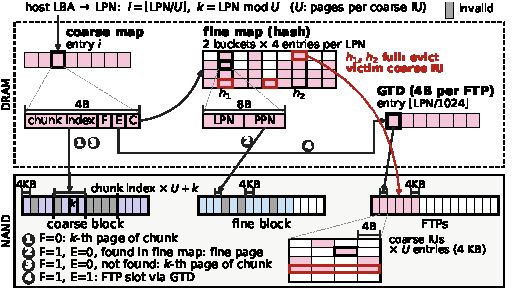
\includegraphics[width=\columnwidth]{figs/fig_design.pdf}
  \vspace{-6mm}
  \caption{DUET mapping structures.}
  \label{fig:design}
  \vspace{-4mm}
\end{figure}

\subsection{Two Mapping Granularities}
\textbf{Coarse map.} The logical space is divided into coarse IUs of $U$ pages
($4U$\,KB), so a logical page number (LPN) belongs to coarse IU $i=\lfloor \mathrm{LPN}/U \rfloor$ at
page offset $k=\mathrm{LPN} \bmod U$. Each coarse IU is stored as a \emph{chunk}
of $U$ physically consecutive, $U$-page-aligned pages in a \emph{coarse block},
and its 4\,B coarse entry holds the chunk index. Since a coarse entry is as large as a page-level
entry, the coarse map takes $1/U$ of the DRAM of a page-level table.

\textbf{Fine map.} A write smaller than a coarse IU is written out of place as 4\,KB
\emph{fine pages} into separate \emph{fine blocks}. The fine map is a two-choice
bucketized hash table~\cite{balanced}. With two candidate
buckets, a bucket fills up much later than in an ordinary hash table with a
single candidate bucket~\cite{balanced}, so DUET evicts entries less often.
% ftlsim (results/coarse_gc/diag, end of run): mean fine pages per flagged IU 1.8 (fio) to 5.0 (YCSB-A) of U = 16,
% d <= 4 for 66-98% of IUs. Per-IU array 16 x 4 B = 64 B per IU vs 8 B x d in the table.
Each 8\,B entry holds an LPN and the
physical page number (PPN) of its fine page. Each LPN has two candidate buckets of four
entries each, and a new entry goes to the less loaded one. The table takes all of
the DRAM budget that the coarse map leaves.
% Implementation (92 GB, 1/8 budget): coarse map 5.6 MB, table 5.5 MB = fine pages of ~3% of logical pages.

The table is similar to cuckoo hashing~\cite{cuckoo} in that each entry has two
candidate buckets. Unlike cuckoo hashing, DUET never moves an existing entry to
its other bucket to make room, so an insert does not trigger a chain of moves.
When both candidate buckets are full, DUET instead writes the fine-map entries
of a victim coarse IU to a \emph{fine translation page} (FTP) in NAND and frees them
from the table (\emph{spill}, Section~\ref{sec:spill}). A table lookup therefore checks at most the eight
entries of the two candidate buckets, and an insert writes into a free entry of
one of them. A spilled entry has a fixed location in NAND, so one map-page
read returns it.

\textbf{Flag bits.} Each coarse entry also has three flag bits. The
\emph{has-fine-pages} (F) bit tells whether the coarse IU has fine pages, the
\emph{spilled} (S) bit tells whether their fine-map entries are in NAND, and the
\emph{clean} (C) bit tells whether the entries in the table are identical to their
copy in NAND (Section~\ref{sec:spill}).

\subsection{Host I/O Path}
\textbf{Read path.} A read first checks the coarse entry of coarse IU $i$. If F is set and S is clear, DUET
looks up the LPN in the fine map. If S is set, the global translation directory
(GTD)~\cite{dftl} locates the FTP of the
LPN, and DUET reads its slot. When the fine map or the slot points to a
fine page, DUET reads the fine page. Otherwise, including when F is clear, it
reads page $k$ of the chunk. A read thus reads at most three DRAM
locations, the coarse entry and the two candidate buckets. A 32\,B bucket lies
within one DRAM row, so each location costs one random DRAM
access~\cite{rixner}. Only a read of a spilled coarse IU adds one map-page read.

\begin{figure}[t]
  \centering
  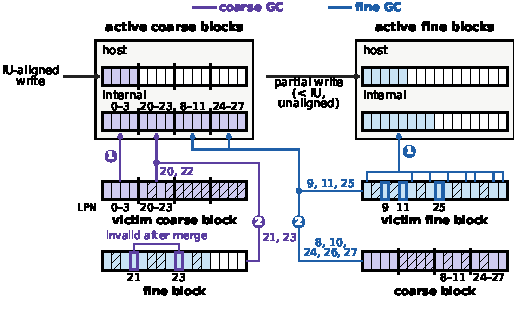
\includegraphics[width=\columnwidth]{figs/fig_write.pdf}
  \vspace{-6mm}
  \caption{DUET write and reclamation paths. Coarse GC (purple) and fine GC (blue) either (1) copy valid data or (2) merge it into new chunks.}
  \label{fig:write}
  \vspace{-4mm}
\end{figure}

\textbf{Write path.} Host writes go to two \emph{active blocks}, an active
coarse block for chunks and an active fine block for fine pages. A host write
is split at coarse-IU boundaries. Each IU-aligned write is written as a new chunk
in the active coarse block. The old chunk and all fine pages of the coarse IU
become invalid, and the corresponding fine-map entries are removed. If the coarse IU
already has fine pages, DUET instead writes the IU-aligned write as fine pages
while the fine blocks are below their cap (Section~\ref{sec:reclaim}).
% fine_full=1: keeps a hot coarse IU in the fine blocks instead of turning it back into a chunk on every full rewrite.

A \emph{partial write}, which is smaller than a coarse IU, is written as fine
pages into the active fine block. For each fine page, DUET inserts its LPN and
PPN into one of the two candidate buckets of the LPN, the less loaded one. The
page of the chunk with the same LPN becomes invalid. If the LPN already has a
fine page, DUET updates the PPN of its fine-map entry instead, and the old fine
page becomes invalid.

DUET keeps fine pages and chunks in different blocks. Fine pages hold recently
rewritten data and chunks hold colder data, and mixing data of different update
frequencies in one NAND block raises the GC cost~\cite{hotcold,dwf,multistream}.
As in other FTLs~\cite{sepbit}, DUET also separates host writes from internal
writes (GC and merges), so it keeps four active blocks (Figure~\ref{fig:write}).
When an active block is full, DUET takes a free block as the new active block.
% Final runs (results/final_vbm, q_vbm2.sh) use coarse_class=0 and uni_onefront=0, i.e. exactly four active blocks.
% Implementation also completes a nearly full partial write as a chunk when cheaper (eager RMW): 0.1-0.8% of host
% programs in the apps, 0 in traces / replays. Not described in the paper.

\subsection{Reclaiming Path}
\label{sec:reclaim}
DUET reclaims a block when the free blocks run low. Its written blocks
are divided into fine blocks, which hold fine pages, and coarse blocks,
which hold chunks.
DUET thus has two kinds of GC. \emph{Fine GC} reclaims a fine block, and
\emph{coarse GC} reclaims a coarse block. To find the valid data of a victim,
DUET keeps a valid bitmap with one bit per chunk slot of the coarse blocks and
one bit per page of the fine blocks.

\textbf{Victim selection.} DUET picks a victim with fewer valid pages to copy, whether it is a coarse
block or a fine block. The number of fine blocks, however, is limited by the OP
space. A fine page makes one page of a chunk invalid, but the chunk still takes
its place in a coarse block. The coarse blocks must therefore be able to cover
the whole logical capacity, and the fine blocks can only use the space beyond
it. When the fine blocks reach this cap, DUET thus reclaims a fine block.
Otherwise, it compares the coarse and fine blocks and runs GC on the side whose
block has fewer valid pages.
% Exact cap: OP blocks - GC reserve (T) - active blocks.
% Implementation: below the cap, the fewest-valid coarse and fine blocks are compared (gc_select_cost=1), and coarse GC
% then picks its actual victim by cost-benefit (not described in the paper).
% Ablation running (2026-11-06): greedy coarse victim on NVMeVirt, results/final_greedy (q_greedy.sh).
% ftlsim (results/coarse_gc pol:g): greedy raises WAF by 7.1% on average (up to 14.8% on TPC-C).

% Dropped (victim policy left implicit, "fewer valid pages to copy" in Victim selection): coarse GC picks its victim by
% cost-benefit [lfs], weighing block age so a recently written block gathers more invalid pages. Fine GC is greedy.
\textbf{Coarse GC.} Coarse GC handles each valid chunk of the victim in
one of two ways (purple lines in Figure~\ref{fig:write}). A chunk whose coarse
IU has no fine pages (LPN 0--3) is copied unchanged to a new chunk (\cgc{1}). A
chunk whose coarse IU has fine pages (LPN 20--23) is only partly valid, so DUET
merges it (\cgc{2}). DUET looks up the LPNs of the coarse IU in the fine map.
An LPN found there has a fine page (LPN 21 and 23), and an LPN not found there
is still valid in the chunk (LPN 20 and 22). DUET reads these pages and writes
them as one merged chunk. The fine pages then become invalid, their fine-map
entries are removed, and the F bit of the coarse IU is cleared.

\textbf{Fine GC.} Fine GC handles each coarse IU with valid fine pages in the victim in one of two ways
(blue lines in Figure~\ref{fig:write}). DUET either copies the fine pages to
another fine block (\fgc{1}) or merges the coarse IU with its chunk (\fgc{2}).
In Figure~\ref{fig:write}, LPN 9 and 11 are merged with the chunk of LPN 8--11,
and LPN 25 with the chunk of LPN 24--27. Let $d$ be the number of fine pages
of the coarse IU in all fine blocks, not only in the victim. A merge reads the
chunk and these $d$ fine pages and writes one new chunk. All $d$ fine pages then
become invalid, and their fine-map entries are removed.

\textbf{Copy-or-merge decision.} DUET chooses one of the two ways by a cost-benefit model. The cost is the
number of pages written, and the benefit is the number of pages freed in the
fine blocks. Let $P$ be the number of pages per block, $v$ the number of valid
pages in the victim, and $U$ the number of pages in a coarse IU. For the same
victim, copying costs $v$ page writes and frees $P - v$ pages. A merge of a
coarse IU with $d$ fine pages instead costs $U$ page writes, one coarse IU, and
frees its $d$ fine pages. The cost-benefit value, that is, the number of pages
freed in the fine blocks per page written, is thus $(P-v)/v$ for copying
(\fgc{1}) and $d/U$ for a merge (\fgc{2}). DUET copies the fine pages when
$(P-v)/v \ge d/U$, and otherwise merges the coarse IU. DUET makes this decision for
every coarse IU that has valid fine pages in the victim fine block.
% Implementation also keeps hot fine pages (cost_cold, rec_block=1): no merge if a fine page of the IU sits in a host
% fine block newer than the victim. Not described in the paper.

Copying fine pages keeps them in the fine blocks, whereas a merge moves them
into a chunk and frees their fine-map entries. The size of the fine map thus
adapts to the workload (Section~\ref{sec:eval}).

\subsection{Fine-Map Spill and Load}
\label{sec:spill}
Under a fixed DRAM budget, the table cannot index every fine page that the fine
blocks can hold. For example, a budget of 128\,MB per TB of capacity, 1/8 of
the page-level table, holds the whole map of an SSD with uniform 32\,KB coarse IUs. If
DUET uses 64\,KB chunks under this budget, the coarse map takes 64\,MB per TB.
Since each fine-map entry takes 8\,B, the remaining 64\,MB holds about 8M
entries, which map 32\,GB of fine pages. If the fine blocks use all of
the 7\% OP space, however, they can hold 70\,GB of fine pages per TB. The table thus has no room for more
than half of their fine-map entries. The DRAM capacity is fixed when the SSD hardware is designed.
Unlike the FTL, which can be updated with the firmware, it cannot be changed easily.
% Illustration: 7% of 1 TB = 70 GB vs 32 GB in the table -> 54% do not fit. (Device: fine cap 18 blocks after GC reserve and active blocks, 1 - 334,736 / 557,568 = 40%.) Per TB: table 334,736 / L 10,798,160 = 3.10% of logical pages = 31.7 GB, fine cap 557,568 / L = 5.16% = 52.9 GB. FAST under the same budget (old text): rwcap=14 of nlog=23, 8 spare blocks unused.
% Numbers: apps device P=30976, fine cap 18 blocks = 557,568 pages, cuckoo2 table 334,736 entries (spill=2, GTD charged).
% FAST (results/final_rp apps dmesg): NB=373 NLB=348 T=2 -> nlog=23, cache_bytes=B12 -> rwcap=14 (SW + 14 RW = 15 log blocks).

Another challenge is hash collisions within the fine map. An insert can find
both of its candidate buckets full even when other buckets still have free slots.
Hashing schemes that place a colliding entry in another
bucket~\cite{cuckoo,onemove,hopscotch,robinhood} make a lookup probe more buckets or an
insert move existing entries, so they need more DRAM accesses. On the other hand,
merging the coarse IU whose entries are pushed out of the full buckets into the coarse map
causes extra NAND writes.

DUET instead keeps the fine-map entries of some coarse IUs in FTPs in NAND, so the
fine blocks can use all of the OP space without more DRAM.
The fine-map entries of a coarse IU move to its FTP when the table fills
(\emph{spill}) and back to the table when the coarse IU is accessed again
(\emph{load}), and no data moves in either direction. In theory, the spilled entries map
at most 7\% of the data, the size of the OP space, because most data are mapped by the
coarse map, which is always in DRAM.
% Bound: spilled <= fine pages <= OP (7%). Spill can start before the table is full (bucket pairs fill unevenly), so
% 70 - 32 GB is not a bound. Measured: YCSB-A max spilled 312,824 / L 10,798,160 = 2.9% (results/final_stats).

\textbf{Spill.} As shown in Figure~\ref{fig:design}, the fine-map entry of each LPN has a
fixed 4\,B slot in an FTP,
which holds the entries of 1024 consecutive LPNs. As in DFTL, the GTD locates each
FTP with one 4\,B entry, charged to the same DRAM budget. When an insert finds both
candidate buckets full, DUET picks a victim among the coarse IUs that have an entry in
the two buckets. It writes all entries of the victim to its FTP, sets its S bit, and
frees its table entries. The other coarse IUs of the same FTP are spilled with the
same program.

\textbf{Load.} An access to a spilled coarse IU reads its FTP and loads only the
entries of that coarse IU into the table. The other
coarse IUs of the FTP stay spilled. A write loads the entries and then updates them.
A read reads the FTP before the data, loads the entries, and sets the C bit of the
coarse IU. The coarse IU stays clean until one of its entries changes.

\textbf{Spill victim.} DUET picks a clean coarse IU first to reduce FTP writes to NAND.
A clean coarse IU is simply dropped from the table and marked spilled because its FTP
copy is still valid. If there is no clean coarse IU, DUET picks the coarse IU with the
most fine pages, so one FTP program frees the most table slots.
% Code: prop_ct_best(pc = spill_rp_clean) prefers clean IUs among the bucket pair, then most fragments, then older.

\textbf{GC.} When GC moves fine pages of spilled coarse IUs, it reads and programs
each FTP at most once per victim block. A merge of a spilled coarse IU reads its
entries from the FTP and then clears its F and S bits.
% Dropped detail (2026-11-06): one recently used FTP is kept in controller SRAM. A coarse IU becomes dirty when one of its
% fine pages changes (write, merge, GC copy).

\subsection{Overhead}
The per-coarse-IU state is the 4\,B coarse entry with its three flag bits, the fine
map is the two-choice hash table, and the GTD adds 4\,B per FTP, all within the budget.
% Valid bitmaps are not charged (prop_mem = NIU*4 + GTD + table slots), as for every other FTL. Not described.
A host read takes at most three DRAM accesses, and a spill or load
touches at most $1024/U$ coarse entries and 1024 table slots.
Mapping reads and programs happen only for spilled coarse IUs and are counted in all
WA and latency results.

% DUET -- Evaluation (DAC 2027 draft, 2026-11-01), rough: figures placed, text to be written.
% Figures: tools/plot_eval.py -> results/paper_dac/fig_eval_{read,write,tput}.pdf, data in results/paper_dac/eval_data.csv.
% Bounded FTLs (DUET, DFTL, LeaFTL, CoMap; uFTL dropped from the figures) = results/final_vbm. Page, FAST, IU+RMW = results/final_rp (traces, apps)
% and results/final_rp_a128 (raw I/O).
% Raw I/O: 4K:128K = 70:30 only, labelled by R:W (2026-11-06). Geomean over the 10 workloads, normalized to Page:
% throughput DUET 0.93, LeaFTL 0.73, DFTL 0.67, IU+RMW 0.66, FAST 0.57, CoMap 0.46.
% Avg. read DUET 1.03, FAST 1.51, IU+RMW 1.61, LeaFTL 1.65, CoMap 1.81, DFTL 2.41.
% Avg. write DUET 0.93, DFTL 0.74, LeaFTL 1.27, FAST 2.40, IU+RMW 2.76, CoMap 3.33.
% p99 read DUET 1.02, FAST 1.35, CoMap 1.67, IU+RMW 1.70, DFTL 1.71, LeaFTL 2.10.
% p99 write DUET 0.75, DFTL 0.71, LeaFTL 0.99, IU+RMW 2.15, FAST 2.50, CoMap 3.65.

\section{Evaluation}
\label{sec:eval}

\textbf{Setup.} TODO: NVMeVirt configuration, OP 7\%, 1/8 mapping DRAM, the seven FTLs, workloads.

\begin{figure*}[t]
  \centering
  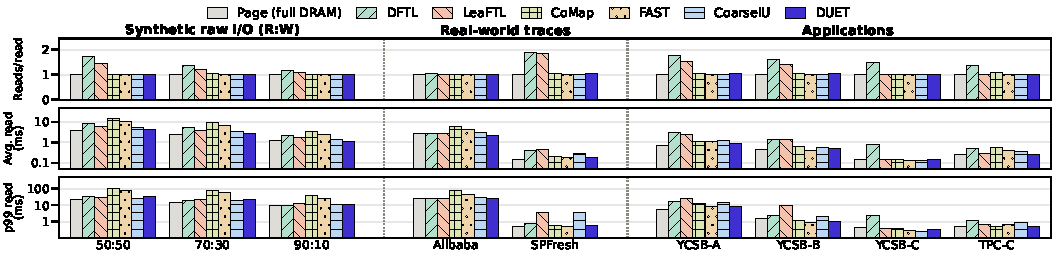
\includegraphics[width=\textwidth]{figs/fig_eval_read.pdf}
  \vspace{-6mm}
  \caption{Read path. From top, flash reads per host read (data plus mapping reads), and average and p99 read latency.}
  \label{fig:eval-read}
  \vspace{-3mm}
\end{figure*}

\begin{figure*}[t]
  \centering
  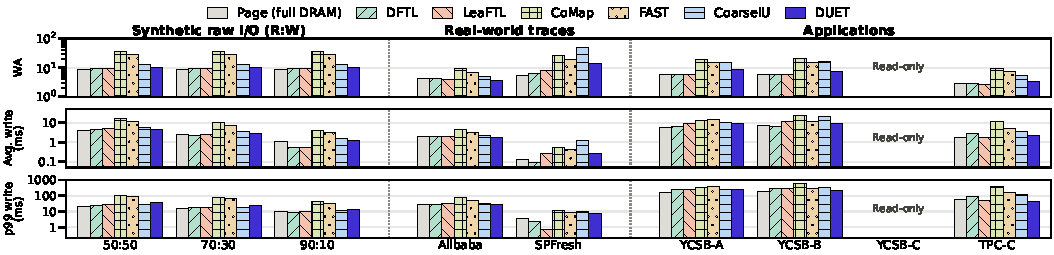
\includegraphics[width=\textwidth]{figs/fig_eval_write.pdf}
  \vspace{-6mm}
  \caption{Write path. From top, device write amplification, and average and p99 write latency.}
  \label{fig:eval-write}
  \vspace{-3mm}
\end{figure*}

\begin{figure*}[t]
  \centering
  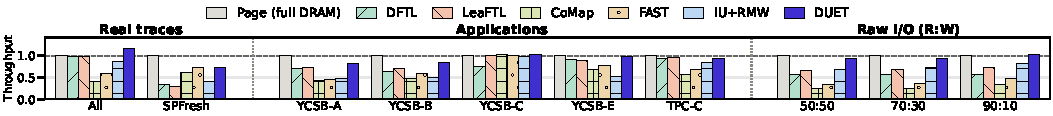
\includegraphics[width=\textwidth]{figs/fig_eval_tput.pdf}
  \vspace{-6mm}
  \caption{Throughput normalized to Page.}
  \label{fig:eval-tput}
  \vspace{-3mm}
\end{figure*}

\textbf{Read latency.} TODO (Figure~\ref{fig:eval-read}).

\textbf{Write amplification and write latency.} TODO (Figure~\ref{fig:eval-write}).

\textbf{Throughput.} TODO (Figure~\ref{fig:eval-tput}).

% Ablation: tools/plot_ablation.py -> results/paper_dac/fig_ablation.{pdf,png}, data in ablation_data.csv.
% Build-up: Basic = nsfm (spill=0, fold_all=1, gc_select_cost=0), + victim selection = nsm, + copy-or-merge = ns,
% + spill/load = DUET (final_vbm). Variants = final_ablation. Normalized to Basic.
\begin{figure}[t]
  \centering
  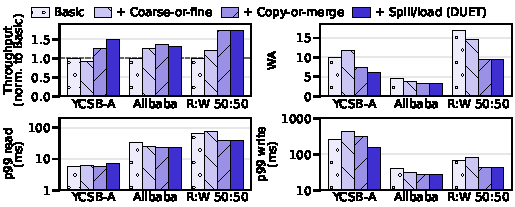
\includegraphics[width=\columnwidth]{figs/fig_ablation.pdf}
  \vspace{-6mm}
  \caption{Ablation. From left to right, each bar adds one more technique to Basic, and the rightmost bar is DUET. Throughput is normalized to Basic.}
  \label{fig:eval-ablation}
  \vspace{-4mm}
\end{figure}

\textbf{Ablation.} TODO (Figure~\ref{fig:eval-ablation}).

% \input{sections/related}
% % DUET -- Conclusion (DAC 2027 draft, 2026-11-07; shortened 2026-11-10)
% Previous version: High-capacity SSDs cannot keep a page-level mapping table in DRAM, and existing FTLs that fit a
% limited DRAM budget slow down either reads or writes. DUET maps most data with coarse IUs and recent small writes with
% 4 KB fine pages. It keeps most of its fine map in DRAM and spills the rest to NAND, and its GC merges fine pages one
% coarse IU at a time. The numbers of its fine blocks and fine-map entries follow the workload. In NVMeVirt with about
% 1/8 of the page-level mapping DRAM, DUET reaches 93% of the throughput of a page-level FTL with unlimited DRAM and
% keeps its read and write latency close to those of that FTL.
\section{Conclusion}
\label{sec:conclusion}
DUET maps most data with coarse IUs and small writes with 4\,KB fine pages, spills
fine-map entries to NAND when its DRAM table fills, and merges fine pages one coarse
IU at a time. With about 1/8 of the page-level mapping DRAM, DUET reaches 93\% of the
throughput of a page-level FTL with unlimited DRAM.


\clearpage
\bibliographystyle{IEEEtran}
\bibliography{refs}

\end{document}
